\documentclass{beamer}
 
\usepackage[frenchb]{babel}
\usepackage[T1]{fontenc}
\usepackage[utf8]{inputenc}
\usepackage{upgreek}
\usepackage{amsmath}
\usepackage{amssymb}
\usepackage{pdfpages}
\usepackage[]{algorithm2e}
\usepackage[abs]{overpic}
\usepackage{mdwlist}
\usepackage{tikz}
\usepackage[style=alphabetic,backend=bibtex,autocite=footnote]{biblatex}

% \bibliographystyle{alpha}
\bibliography{../../articles/biblio.bib}
\nocite{*}

\usetheme{Frankfurt}
  
\title{La phylogénie des images dans les réseaux sociaux}
\author{Noé LE PHILIPPE}
\institute{Équipe ICAR - William Puech}
\date{\today}
% \logo{\includegraphics[height=10mm]{images/logo.png}}

\addtobeamertemplate{navigation symbols}{}{%
    \usebeamerfont{footline}%
    \usebeamercolor[fg]{footline}%
    \hspace{1em}%
    \insertframenumber/\inserttotalframenumber
}

\AtBeginSection[]
{
  \begin{frame}
  \frametitle{Sommaire}
  \tableofcontents[currentsection, hideothersubsections]
  \end{frame} 
}

\makeatletter
\renewcommand\@makefnmark{\hbox{\@textsuperscript{\normalfont[\@thefnmark]}}}
\renewcommand\@makefntext[1]{{\normalfont[\@thefnmark]}\enspace #1}
\makeatother

\DeclareCiteCommand{\footfullcitetext}[\mkbibfootnotetext]
{\usebibmacro{prenote}}
{\usedriver
  {\DeclareNameAlias{sortname}{default}}
  {\thefield{entrytype}}}
{\multicitedelim}
{\usebibmacro{postnote}}

\newenvironment<>{varblock}[2][.9\textwidth]{%
  \setlength{\textwidth}{#1}
  \begin{actionenv}#3%
    \def\insertblocktitle{#2}%
    \par%
    \usebeamertemplate{block begin}}
  {\par%
    \usebeamertemplate{block end}%
  \end{actionenv}}

\begin{document}

\begin{frame}
  \titlepage
\end{frame}

\section{Le sujet de stage}
\begin{frame}
  \frametitle{Le sujet de stage}

  \begin{block}{Le sujet}
    La phylogénie des images dans les réseaux sociaux
  \end{block}

  \begin{block}{Définition}
    {\large ``La phylogenèse ou phylogénie est l'étude des relations de parenté entre êtres vivants.''}
    \hspace*\fill{\small--- Wikipedia}
  \end{block}

\end{frame}

\begin{frame}
  \frametitle{Les applications}
  \begin{block}{}
    Réduire le nombre de versions de la même image pour optimiser l'espace de stockage
  \end{block}
  \pause
  \begin{block}{}
    Suivre l'évolution et la diffusion d'images sur les réseaux sociaux
  \end{block}
  \pause
  \begin{block}{}
    Détecter l'altération d'images
  \end{block}
\end{frame}

\begin{frame}
  \frametitle{Définitions}

  \begin{block}{Near-Duplicate Image (NDI)}
    Une image I\textsubscript{1} est le near-duplicate\footnotemark\ d'une image I si :
    $$I_{1} = T(I), T \in \mathcal{T}$$
    où $\mathcal{T}$ est un ensemble de transformations autorisées
  \end{block}\footfullcitetext{joly2007content}
  Dans le cas général, 
  \begin{multline*}
    \mathcal{T} = \{resampling, cropping, affine\ warping,\\ color\ changing, lossy\ compression\}
  \end{multline*}
  mais dans le cadre du stage, $\mathcal{T} = \{lossy\ compression\}$
\end{frame}

\begin{frame}
  \frametitle{Définitions}
  \begin{block}{Image Phylogeny Tree (IPT)}
    C'est l'arbre retraçant la parenté des images
  \end{block}

  \begin{center}
      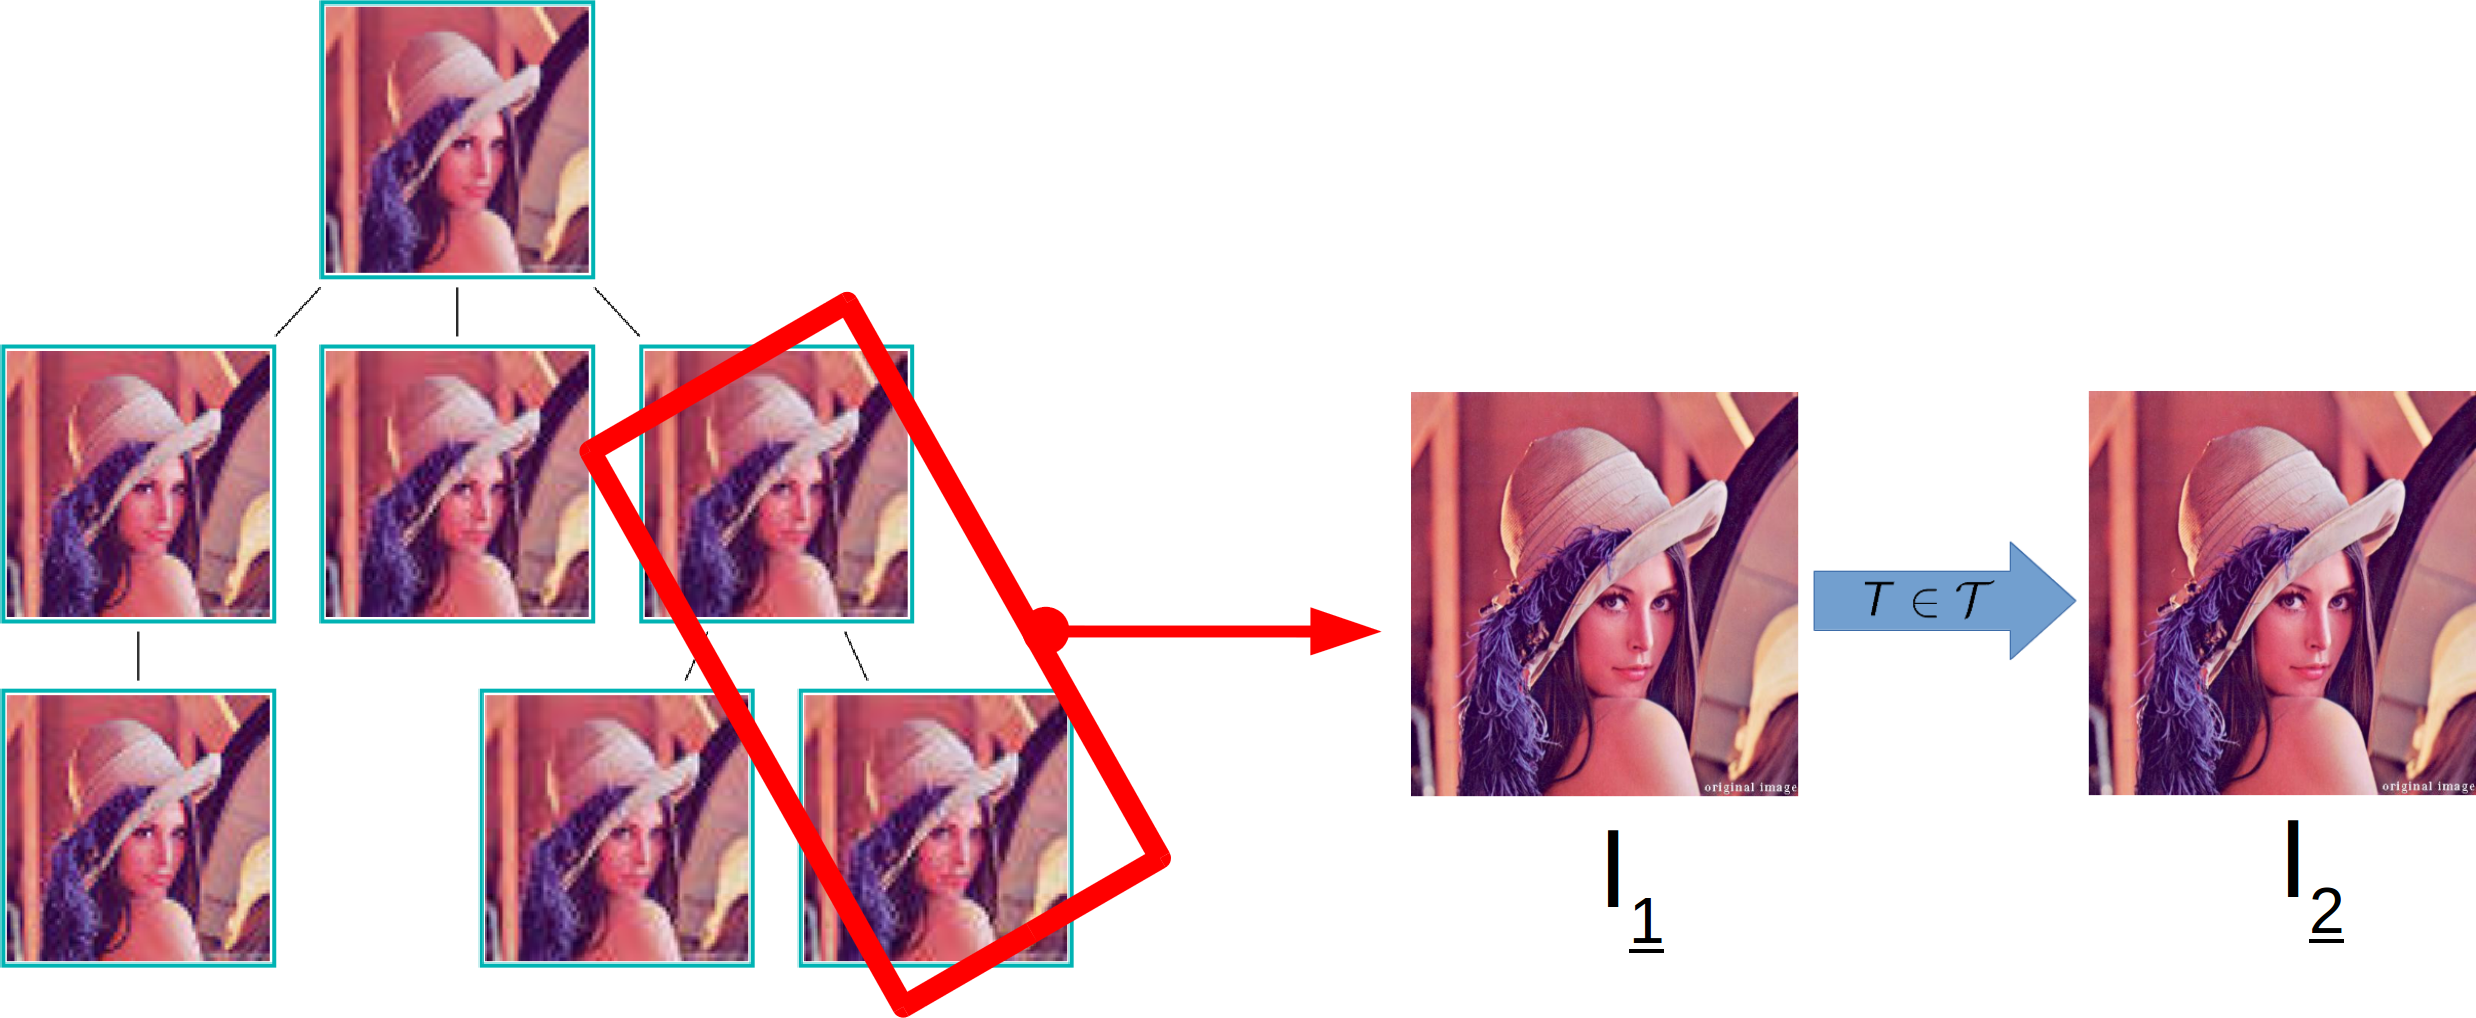
\includegraphics[width=1\textheight]{tree_extract.png}
  \end{center}

\end{frame}

\begin{frame}
  \frametitle{Image phylogeny tree}
  \begin{center}
    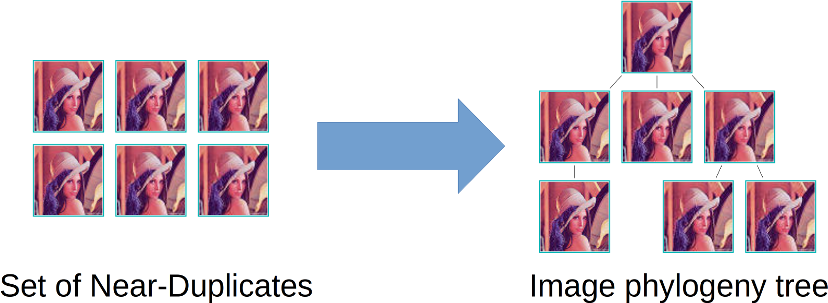
\includegraphics[width=0.8\textwidth]{set_to_tree.png}
  \end{center}
  Deux parties importante lors de la reconstruction de l'arbre phylogénétique : 
  \pause
  \begin{columns}
    \begin{column}{0.5\textwidth}
      \begin{block}{}
        \begin{itemize}
        \item Correctement identifier la racine
        \end{itemize}
      \end{block}
      \pause
    \end{column}
    \begin{column}{0.5\textwidth}
      \begin{block}{}
        \begin{itemize}
        \item Estimer au mieux l'arborescence
        \end{itemize}
      \end{block}
    \end{column}
  \end{columns}
\end{frame}

\section{État de l'art}

\begin{frame}
  \frametitle{Du plus ancien}

\only<1,3,5> {
  \begin{block}{Visual Migration Map}
    \begin{itemize}
    \item Les transformations sont directionnelles
    \item Relation parent-enfant si tous les détecteurs s'accordent sur la direction
    \item Simplification du graphe par sélection des plus longs chemins
    \end{itemize}
  \end{block}
  \footfullcite{kennedy2008internet}
}
  \only<2> {
    \begin{center}
      \includegraphics<2>[scale=0.3]{vmm}
    \end{center}
  }
  \only<4> {
    \begin{center}
    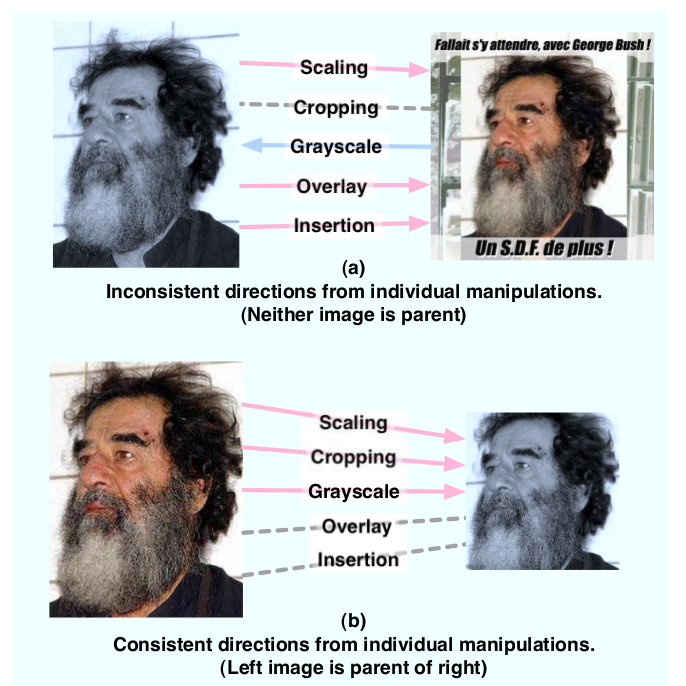
\includegraphics[scale=0.3]{vmm_directionnel}
    \end{center}
  }
  \only<6> {
    \begin{center}
    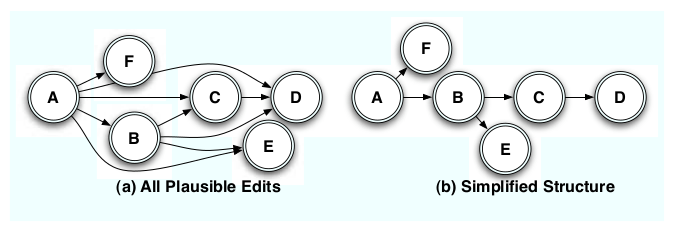
\includegraphics[scale=0.45]{vmm_tree}
    \end{center}
  }
\end{frame}

\begin{frame}
  \frametitle{Au plus récent}
  \begin{block}{Image phylogeny tree}
    \begin{itemize}
      \item Calcul d'une \textit{dissimilarity matrix}
      \item Calcul d'un arbre couvrant de poids min (Kruskal ou autre)
    \end{itemize}
  \end{block}
  \footfullcite{dias2010first}
  \footfullcite{dias2012image}
\end{frame}

\section{Analyse des recompressions}
\begin{frame}
  \frametitle{Convergence des blocs lors de compressions successives}
  \begin{block}{But}
    Compter le nombre de compressions
  \end{block}
  \begin{block}{3 types de blocs}
    \begin{itemize}
      \item Les blocs plats
      \item Les blocs stables
      \item Les blocs cycliques
    \end{itemize}
  \end{block}  
  \begin{block}{Comment ?}
    plus petit commun multiple de la longueur des cycles
  \end{block}
  \footfullcite{CarneinSB2016TelltaleWatermarks}
\end{frame}

\begin{frame}
  \frametitle{Convergence des blocs lors de compressions successives}
   
    \only<1,3>{
      \begin{block}{Utilisation des blocs}
        \begin{itemize}
        \item Les blocs de l'image
        \item Insérer des blocs
        \end{itemize}
      \end{block}
      \pause
      \begin{block}{Les inconvénients}
        \begin{itemize}
        \item Nécessite du padding
        \item Limité à la même table de quantification
        \item Résultats moyens pour Q < 100
        \end{itemize}
      \end{block}  
    }

  \only<2> {
    \begin{center}
      \includegraphics<2>[scale=0.3]{insertion_blocs}
    \end{center}
  }
  \footfullcite{CarneinSB2016TelltaleWatermarks}
\end{frame}

\begin{frame}
  \frametitle{Estimation de la matrice de compression primaire}
  \only<1,3>{
    \begin{block}{Analyse des valeurs manquantes de l'histogramme}
      Artefacts distincts pour $Q^{1} > Q^{2}$ et $Q^{1} < Q^{2}$
    \end{block}
    \pause
    \begin{block}{Limites}
      \begin{itemize}
      \item $Q^{1} = Q^{2}$
      \item $Q^{1}$ est facteur de $Q^{2}$
      \end{itemize}
    \end{block}
  }
  \only<2> {
    \begin{figure}
      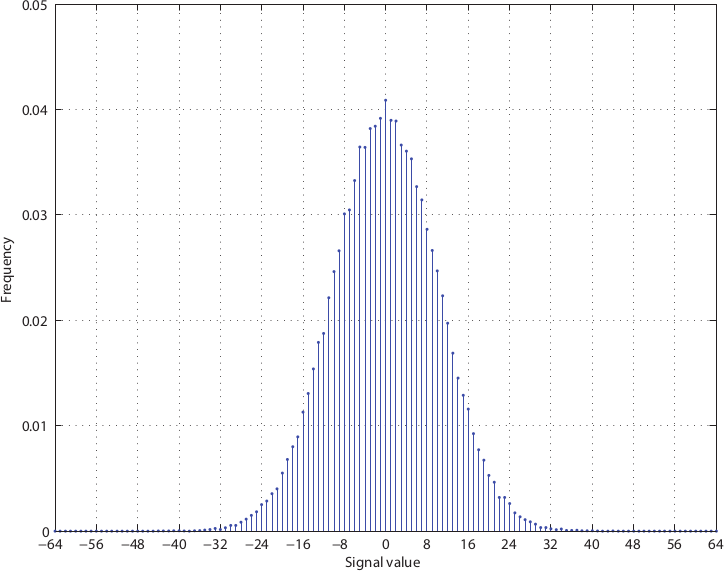
\includegraphics[height=0.4\textheight]{h1}
      \hfill
      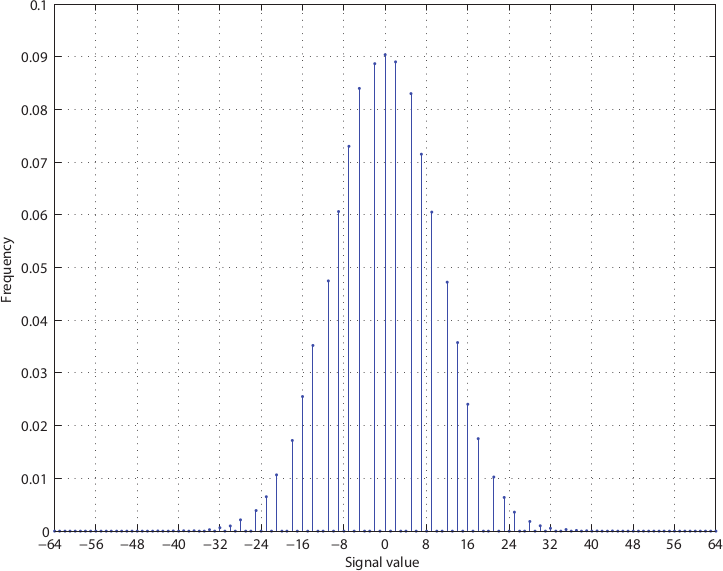
\includegraphics[height=0.4\textheight]{h2}
    \end{figure}
    \begin{figure}
      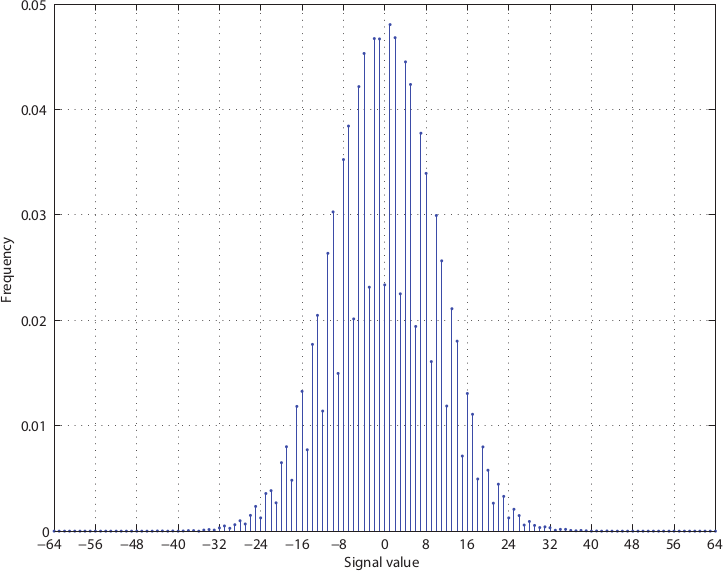
\includegraphics[height=0.4\textheight]{h3}
    \end{figure}
  }
\end{frame}

% \begin{frame}
%   \frametitle{Estimation de la matrice de compression primaire}
%   \begin{block}{Analyse des valeurs manquantes de l'histogramme}
%     Artefacts distincts pour $Q^{1} > Q^{2}$ et $Q^{1} < Q^{2}$
%   \end{block}
%   \pause
%   \begin{block}{Limites}
%     \begin{itemize}
%     \item $Q^{1} \neq Q^{2}$
%     \item $Q^{1}$ n'est pas facteur de $Q^{2}$
%     \end{itemize}
%   \end{block}
% \end{frame}

\begin{frame}
  \frametitle{Estimation de la matrice de compression primaire}
  \begin{block}{Principe de leur méthode}
    Comparer l'histogramme de l'image originale et l'histogramme des images compressées avec des tables de quantification modèles puis compressées avec $Q^{2}$ et enfin garder la table pour laquelle la différence entre histogramme est la plus faible
  \end{block}
  % \begin{enumerate}
    
  % \item Extraire la table de quantification $Q^{2}$
  %   % \end{enumerate}
  %   \suspend{enumerate}
  %   Pour tous les coefficients intéressants
  %   % \begin{enumerate}[resume]
  %   \resume{enumerate}
  % \item Obtenir l'histogramme $h_{0}$ des valeurs absolues des coefficients DCT de l'image
  % \item Crop l'image (par 4 et 4 pixels)
  % \item Sélectionner les matrices de quantification $Q^{1,1},...,Q^{1,n}$ pour chaque valeur candidate de la matrice primaire
  % \item Compresser l'image cropée avec les matrices $Q^{1,1},...,Q^{1,n}$
  % \item Décompresser toutes les images obtenue et les compresser avec $Q^{2}$

  % \end{enumerate}

\end{frame}

\section{Notre approche}
\begin{frame}
  \frametitle{Notre approche}
  \begin{block}{Matrice de parenté}
    \begin{itemize}
    \item Tentative de preuve qu'une image n'est pas le parent d'une autre
    \item Si c'est impossible, l'image doit alors être le parent
    \item Extraction d'une \textit{matrice de parenté}
    \item Calcul de l'arbre
    \end{itemize}
  \end{block}
\end{frame}

\begin{frame}
  \frametitle{Calcul de l'IPT}
\scalebox{0.75}{%
  \begin{algorithm}[H]
    \LinesNumbered
    \KwData{M a n*n parentage matrix}
    \KwResult{the root of the tree}
    \BlankLine
    $nextRoot \leftarrow$ row with min sum of elements\;
    $treeRoot \leftarrow nextRoot$\;
    \BlankLine

    \ForAll{rows row of M}{
      $root \leftarrow nextRoot$\;
      mark $root$ as done\;
      \BlankLine
      \For{$i\leftarrow 0$ \KwTo n}{
        $row[i] \leftarrow 0$\;
        \If{sum of elements of row == 0} {
          add $i$ as child of $root$\;
        }
        \If{row has the smallest sum of elements and is not marked as done} {
          $nextRoot \leftarrow i$\;
        }
      }
    }
    \KwRet treeRoot
\end{algorithm}}
\end{frame}

\begin{frame}
  \frametitle{La suite}
  \begin{block}{La problématique}
    Identifier un ensemble de marqueurs qui permettraient de réfuter qu'une image est le parent d'une autre
  %   \begin{itemize}
  %   \item Réduction d'un problème de reconstruction d'un arbre de phylogénie à un problème de négation de parenté
  %   \item Utilisation des techniques dans le domaine du forensic
  %   \end{itemize}
  \end{block}
  \begin{block}{Les pistes}
    \begin{itemize}
      \item Distance entre les histogrammes des coefficients DCT
      \item Valeurs manquantes à cause des compressions successives
    \end{itemize}
  \end{block}
  \begin{block}{Point clé}
    Réduction d'un problème de reconstruction d'un arbre de phylogénie à un problème de négation de parenté
  \end{block}
\end{frame}

\begin{frame}
  \frametitle{La suite}
  \begin{center}
    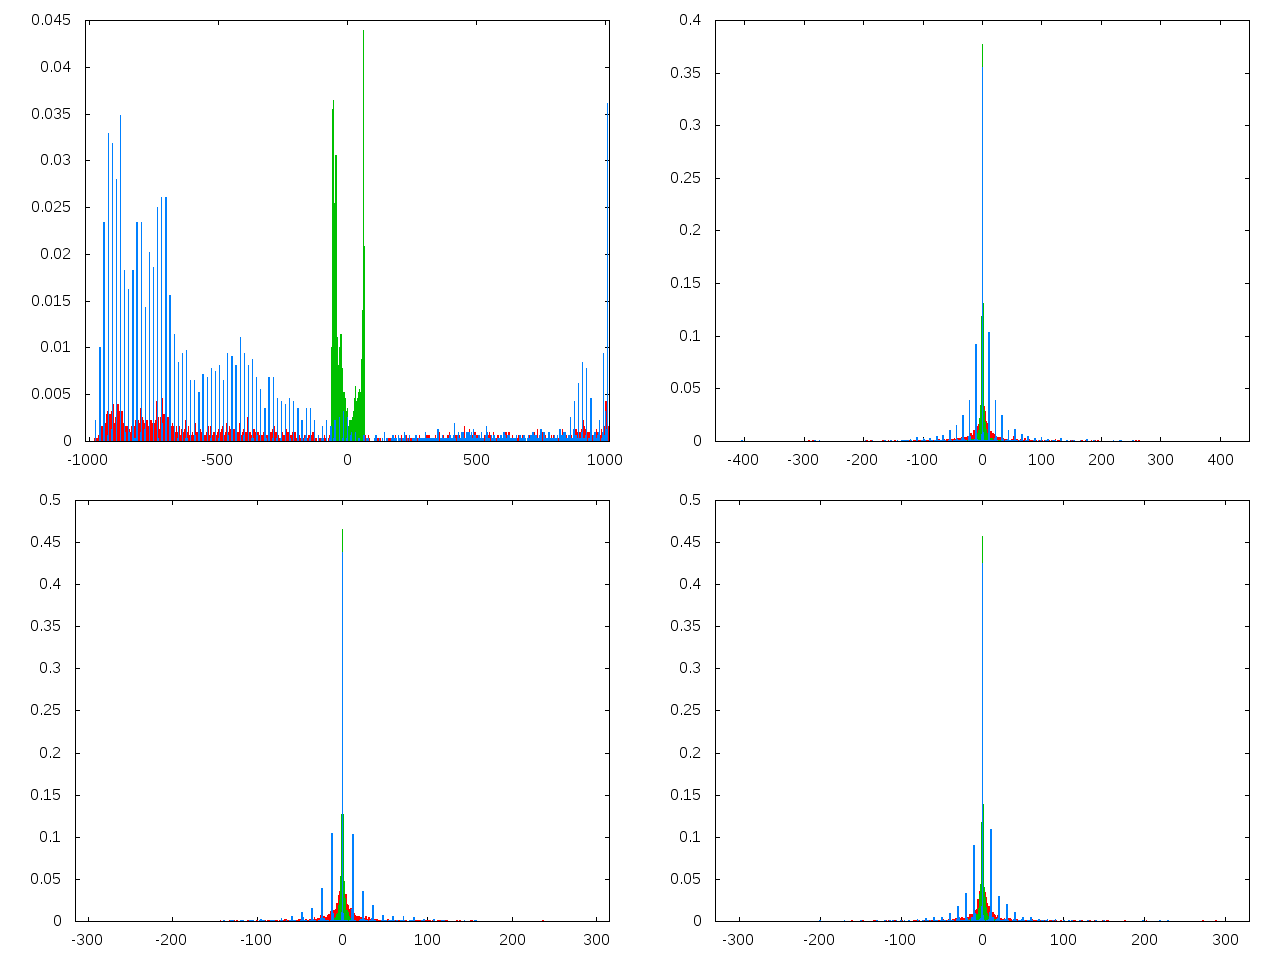
\includegraphics[width=100mm]{out.png}
  \end{center}
\end{frame}
\end{document}

